% Bản tiếng Việt song song với main.tex (cùng cấu trúc, cùng bảng và hình). Biên dịch bằng xelatex.
\documentclass[10pt,twocolumn,letterpaper]{article}

\usepackage{wacv}
\usepackage{fontspec}
\setmainfont{texgyretermes-regular.otf}[Path=/home/tan/.TinyTeX/texmf-dist/fonts/opentype/public/tex-gyre/,BoldFont=texgyretermes-bold.otf,ItalicFont=texgyretermes-italic.otf,BoldItalicFont=texgyretermes-bolditalic.otf]
\font\elvbf="[/home/tan/.TinyTeX/texmf-dist/fonts/opentype/public/tex-gyre/texgyretermes-bold.otf]:mapping=tex-text" at 11pt
\font\tenbf="[/home/tan/.TinyTeX/texmf-dist/fonts/opentype/public/tex-gyre/texgyretermes-bold.otf]:mapping=tex-text" at 10pt

%
% --- inline annotations
%
\newcommand{\red}[1]{{\color{red}#1}}
\newcommand{\todo}[1]{{\color{red}#1}}
\newcommand{\TODO}[1]{\textbf{\color{red}[TODO: #1]}}
% --- disable by uncommenting  
% \renewcommand{\TODO}[1]{}
% \renewcommand{\todo}[1]{#1}


\usepackage{booktabs}
\usepackage{multirow}
\usepackage{amsmath}
\usepackage{graphicx}
\graphicspath{{figs/}}

\definecolor{wacvblue}{rgb}{0.21,0.49,0.74}
\usepackage[pagebackref,breaklinks,colorlinks,allcolors=wacvblue]{hyperref}
\usepackage[capitalize]{cleveref}
\renewcommand{\figurename}{Hình}
\renewcommand{\tablename}{Bảng}
\renewcommand{\refname}{Tài liệu tham khảo}
\renewcommand{\abstractname}{Tóm tắt}
\newcommand{\crefpairconjunction}{ và }\newcommand{\crefmiddleconjunction}{, }\newcommand{\creflastconjunction}{ và }
\newcommand{\crefpairgroupconjunction}{ và }\newcommand{\crefmiddlegroupconjunction}{, }\newcommand{\creflastgroupconjunction}{ và }
\renewenvironment{abstract}{\thispagestyle{empty}\centerline{\large\bf Tóm tắt}\vspace*{12pt}\noindent\it\ignorespaces}{\par\vspace*{12pt}}
\crefname{figure}{Hình}{Hình}\Crefname{figure}{Hình}{Hình}
\crefname{table}{Bảng}{Bảng}\Crefname{table}{Bảng}{Bảng}
\crefname{section}{Mục}{Mục}\Crefname{section}{Mục}{Mục}
\crefname{subsection}{Mục}{Mục}\Crefname{subsection}{Mục}{Mục}
\crefname{appendix}{Phụ lục}{Phụ lục}\Crefname{appendix}{Phụ lục}{Phụ lục}
\crefname{equation}{công thức}{công thức}\Crefname{equation}{Công thức}{Công thức}

\def\wacvPaperID{*****}
\def\confName{WACV}
\def\confYear{2027}
\newcommand{\pts}{\,điểm}

\title{Complementary Foundation Encoders and Prior-Corrected Thresholds\\for Cross-Domain Pedestrian Attribute Recognition\\[4pt]
\large (Bản tiếng Việt để đối chiếu)}

\author{Nhóm tác giả ẩn danh\\
UPAR Challenge 2027, Track 1}

\begin{document}
\maketitle

%=====================================================================
\begin{abstract}
Mô hình nhận dạng thuộc tính người đi bộ thường được huấn luyện trên dữ liệu của một số camera rồi đem dùng ở camera khác. Giữa các camera có khác biệt về domain (tạm dịch: miền dữ liệu). Độ phân giải, góc nhìn và ánh sáng thay đổi, và mỗi bộ dữ liệu còn gán nhãn theo quy ước riêng. Các foundation model (tạm dịch: mô hình nền tảng) được pretrain trên lượng ảnh rất lớn và đa dạng, nên đặc trưng của chúng ít phụ thuộc vào một domain cụ thể. Khi fine-tune trên vài bộ dữ liệu giám sát, mô hình lại dễ học theo đặc điểm và quy ước của chính các bộ đó, làm mất một phần khả năng tổng quát này. Chúng tôi đề xuất một hệ thống giữ lại khả năng đó và sửa cách ra quyết định. Thứ nhất, chúng tôi kết hợp hai foundation model pretrain theo hai cách khác nhau, DINOv3 học chỉ từ ảnh và CLIP học từ ảnh kèm chú thích. Mỗi mô hình chỉ được fine-tune ở các tầng trên cùng, rồi kết quả của hai mô hình được lấy trung bình. Do pretrain khác nhau, hai mô hình mắc lỗi khác nhau trên domain mới, nên trung bình của chúng chính xác hơn từng mô hình. Thứ hai, chúng tôi hiệu chỉnh ngưỡng quyết định. Ngưỡng 0.5 tối ưu cho độ chính xác trên dữ liệu huấn luyện, trong khi metric của cuộc thi chấm cân bằng giữa mẫu có và mẫu không có thuộc tính, và tần suất thuộc tính ở domain mới lại khác. Hệ quả là các thuộc tính hiếm bị dự đoán thiếu. Chúng tôi dịch ngưỡng của mỗi thuộc tính theo tần suất của nó, với một hệ số chung cho cả 40 thuộc tính. Lượng dịch suy ra từ công thức tính điểm, nên không cần nhãn của domain mới. Trên một bộ dữ liệu giữ lại để mô phỏng domain mới, hai thành phần cùng nhau tăng 1.8 điểm so với mô hình đơn tốt nhất. Hệ thống đạt 0.7997 Challenge\_Avg trên tập test ẩn của UPAR 2027 Track~1.
\end{abstract}

\begin{figure*}[t]
\centering
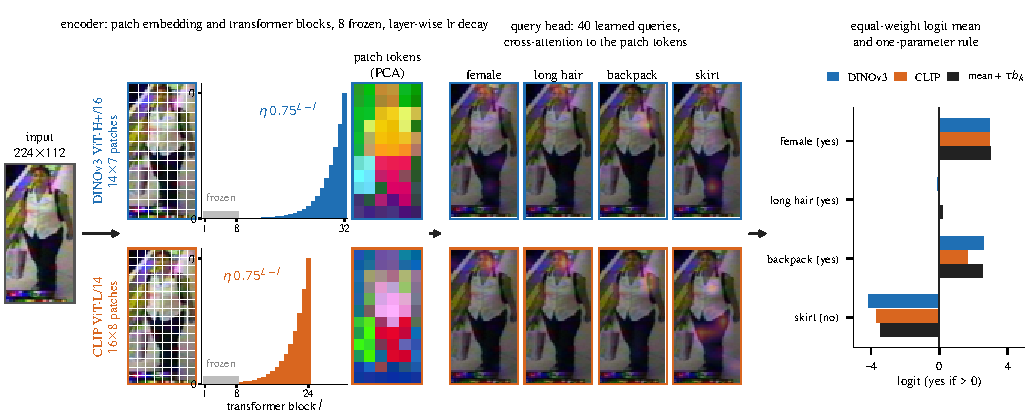
\includegraphics[width=\linewidth]{architecture.pdf}
\caption{Tổng quan phương pháp trên một ảnh PETA. Mỗi hàng là một encoder, gồm lưới patch, learning rate của từng block transformer khi fine-tune, và các patch token được tô màu theo ba thành phần chính đầu tiên. Query của mỗi thuộc tính chú ý vào các token, rồi logit của hai encoder được lấy trung bình và dịch theo phép hiệu chỉnh prior. Token, attention và logit lấy từ các thành viên ViT-L chưa từng thấy PETA khi huấn luyện.}
\label{fig:arch}
\end{figure*}

%=====================================================================
\section{Giới thiệu}
\label{sec:intro}

Pedestrian attribute recognition (PAR, tạm dịch: nhận dạng thuộc tính người đi bộ) dự đoán các đặc điểm như giới tính, màu quần áo và đồ mang theo từ ảnh cắt của một người. Bài toán này phục vụ các truy vấn như ``một phụ nữ mặc áo hồng đeo ba lô'' trong video giám sát. Trong thực tế, mô hình chạy trên những camera không nằm trong dữ liệu huấn luyện. Các benchmark chuẩn~\cite{peta,pa100k,market} không kiểm tra được trường hợp này, vì ảnh huấn luyện và ảnh test của chúng lấy từ cùng các camera. Các kỳ UPAR challenge~\cite{upar,upar23,upar24} thì kiểm tra được. Chúng huấn luyện trên vài bộ dữ liệu công khai và test trên một domain không đóng góp ảnh huấn luyện nào.

Khi mô phỏng tình huống này bằng cách giữ lại một bộ dữ liệu huấn luyện, chúng tôi thấy hai vấn đề tách biệt. Thứ nhất, khả năng xếp hạng kém đi. AUC trung bình của một encoder mạnh giảm khoảng bốn điểm trên bộ dữ liệu giữ lại. Ảnh dương và ảnh âm vì thế bị tách bạch kém hơn. Thứ hai, ngưỡng không còn phù hợp. Challenge dùng ngưỡng cố định 0.5, trong khi tần suất các thuộc tính ở domain mới khác với dữ liệu huấn luyện. Nếu chỉnh ngưỡng bằng chính nhãn của bộ giữ lại thì điểm tăng thêm khoảng ba điểm. Con số đó cho thấy ngưỡng cố định gây mất bao nhiêu.

Chúng tôi đề xuất một thành phần cho mỗi vấn đề (\cref{fig:arch}). Để cải thiện xếp hạng, chúng tôi kết hợp hai encoder có cách pretrain khác nhau. DINOv3~\cite{dinov3} học chỉ từ ảnh, còn CLIP~\cite{clip} học từ ảnh đi kèm văn bản. Lỗi của chúng trên domain mới khác nhau, nên lấy trung bình sẽ có lợi. Cả hai chỉ được fine-tune ở các block phía trên, để giữ lại phần lớn đặc trưng đã pretrain. Để sửa ngưỡng, chúng tôi cộng vào mỗi logit một lượng hiệu chỉnh phụ thuộc vào tần suất của thuộc tính trong dữ liệu huấn luyện. Lượng hiệu chỉnh được suy ra từ phần balanced accuracy của metric, mà điểm tối ưu của phần này không phụ thuộc vào tần suất thuộc tính ở domain mới. Toàn bộ 40 thuộc tính dùng chung một hệ số tự do.

Các đóng góp của bài gồm:
\begin{itemize}
\item Một hệ thống hai encoder cho PAR khác domain. Hệ thống ghép một foundation encoder tự giám sát với một foundation encoder học từ ảnh và văn bản, mỗi encoder có một query head, rồi lấy trung bình logit (\cref{sec:encoders,sec:ensemble}).
\item Một phép hiệu chỉnh ngưỡng theo prior với một hệ số duy nhất, suy ra từ metric của challenge. Phép hiệu chỉnh không cần nhãn của domain đích và chuyển sang domain mới tốt hơn ngưỡng riêng từng thuộc tính chỉnh trên dữ liệu huấn luyện (\cref{sec:rule,sec:exp_rule}).
\item Một khảo sát các lựa chọn thiết kế quan trọng trên camera chưa thấy. Khảo sát chỉ ra cách chọn encoder đi cặp, cách kết hợp các encoder và nên fine-tune sâu đến đâu (\cref{sec:exp_partner,sec:exp_design,sec:exp_depth}).
\end{itemize}
Hệ thống đạt 0.7997 Challenge\_Avg trên tập test ẩn của UPAR 2027 Track~1.

%=====================================================================
\section{Các công trình liên quan}
\label{sec:related}

\paragraph{Nhận dạng thuộc tính người đi bộ.} DeepMAR~\cite{deepmar} coi PAR là bài toán phân loại đa nhãn và đánh trọng số loss theo tần suất thuộc tính. Các phương pháp sau đó thêm module để định vị thuộc tính hoặc mô hình hoá quan hệ giữa chúng. Jia và cộng sự~\cite{rethinkpar} cho thấy nhiều phần tăng này biến mất khi dùng cách chia dữ liệu đánh giá chặt hơn. Query-based head (tạm dịch: đầu phân loại dạng truy vấn)~\cite{q2l,mldecoder} cho mỗi nhãn một query học được trên các token của ảnh, và chúng tôi dùng một head như vậy. UPAR~\cite{upar} thống nhất bốn bộ dữ liệu về chung 40 thuộc tính, nhờ đó đánh giá khác domain trở nên khả thi.

\paragraph{Encoder pretrain khi đổi domain.} Với một backbone mạnh, huấn luyện thông thường đã ngang các phương pháp domain generalization (tạm dịch: tổng quát hoá sang domain mới) chuyên biệt~\cite{domainbed}. Fine-tune toàn bộ mạng có thể làm méo đặc trưng đã pretrain và giảm độ chính xác khi phân phối dữ liệu thay đổi~\cite{lpft}. Điều này là động lực cho fine-tune một phần và cho việc nội suy với trọng số pretrain~\cite{wiseft}. Lấy trung bình trọng số của nhiều mô hình đã fine-tune cũng làm tăng độ bền~\cite{soups,diwa}.

\paragraph{Ensemble.} Một ensemble tốt lên khi các thành viên chính xác và khi chúng mắc lỗi khác nhau~\cite{krogh}. Deep ensemble thuộc nhóm mô hình đáng tin cậy nhất khi tập dữ liệu thay đổi~\cite{deepens,ovadia}. Chúng tôi khảo sát yếu tố nào trong hai yếu tố trên quan trọng khi thành viên là foundation encoder và metric dùng ngưỡng cố định.

\paragraph{Hiệu chỉnh theo prior.} Khi tần suất các lớp thay đổi, xác suất dự đoán có thể được hiệu chỉnh bằng tỉ số giữa các tần suất~\cite{saerens,lipton}. Cộng thêm log prior có hệ số vào logit sẽ tối ưu sai số cân bằng~\cite{logitadj}. Phép hiệu chỉnh ngưỡng của chúng tôi dựa trên ý tưởng này và còn khử phần dịch do trọng số loss của DeepMAR gây ra.

%=====================================================================
\section{Phương pháp}
\label{sec:method}

\subsection{Bài toán và metric}
\label{sec:task}

Mỗi ảnh cắt có 40 thuộc tính nhị phân. Chúng bao gồm tuổi (ba lớp), giới tính, độ dài tóc (ba lớp), độ dài tay áo, độ dài và kiểu của quần váy, mười hai màu thân trên, mười hai màu thân dưới và năm loại phụ kiện. Điểm của challenge là Challenge\_Avg (Avg), trung bình điều hoà của hai thành phần. Thành phần thứ nhất là mA, balanced accuracy (tạm dịch: độ chính xác cân bằng) lấy trung bình trên các thuộc tính. Thành phần thứ hai là instance F1, điểm F1 của tập thuộc tính dự đoán cho từng ảnh, lấy trung bình trên các ảnh. Cả hai thành phần đều cắt xác suất dự đoán ở ngưỡng 0.5.

\subsection{Hai encoder bổ trợ nhau}
\label{sec:encoders}

Một encoder đơn lẻ mắc lỗi có hệ thống trên domain mới. Hai encoder chỉ giúp được nhau nếu lỗi của chúng khác nhau, và lỗi khác nhau nhiều nhất khi hai encoder được pretrain theo cách khác nhau. Vì vậy chúng tôi ghép DINOv3 ViT-H+/16~\cite{dinov3}, học bằng self-distillation (tạm dịch: tự chưng cất) trên ảnh, với CLIP ViT-L/14~\cite{clip}, học cách khớp ảnh với chú thích. Cả hai đọc ảnh cắt kích thước $224\times112$, cho $14\times7$ patch token ở DINOv3 và $16\times8$ ở CLIP.

Fine-tune trên ba bộ dữ liệu huấn luyện chỉ nên thay đổi đặc trưng pretrain ở mức cần thiết. Chúng tôi đóng băng lớp patch embedding và tám block transformer đầu tiên. Các block còn lại dùng layer-wise learning-rate decay (tạm dịch: giảm learning rate theo tầng)~\cite{beit}, nên block thứ $l$ trong $L$ block nhận learning rate $\eta\cdot0.75^{L-l}$. \Cref{fig:arch} vẽ các learning rate này. Phần lớn cập nhật diễn ra ở vài block cuối.

\paragraph{Query head.} Mỗi thuộc tính phụ thuộc vào vùng riêng của nó, ví dụ khuôn mặt với kính hoặc phần chân với váy. Chúng tôi dùng query head~\cite{q2l,mldecoder}, trong đó mỗi thuộc tính có một vector query học được. Query này chú ý vào các patch token qua một tầng cross-attention (tạm dịch: chú ý chéo) tám head, sau đó một MLP nhỏ và bộ phân loại riêng của thuộc tính đó cho ra logit. \Cref{fig:arch} cho thấy các query tập trung vào đúng vùng của thuộc tính, kể cả trên bộ dữ liệu mà encoder chưa từng thấy.

\paragraph{Hàm loss khi huấn luyện.} Chúng tôi dùng binary cross-entropy với label smoothing (tạm dịch: làm mềm nhãn) 0.05 và trọng số DeepMAR~\cite{deepmar}, gồm $w_k^{+}=e^{1-\pi_k}$ cho mẫu dương và $w_k^{-}=e^{\pi_k}$ cho mẫu âm. Ở đây $\pi_k$ là tần suất của thuộc tính $k$ trong nhãn huấn luyện. Các trọng số này làm thuộc tính hiếm được tính nặng hơn. Chúng cũng làm dịch quyết định của mô hình, và phép hiệu chỉnh ngưỡng ở \cref{sec:rule} có tính đến phần dịch này. Các bộ dữ liệu được lấy mẫu theo tỉ lệ căn bậc hai kích thước, để bộ lớn nhất không lấn át. \Cref{app:config} liệt kê toàn bộ thiết lập.

\subsection{Lấy trung bình logit}
\label{sec:ensemble}

Hai encoder cho mỗi thuộc tính một logit, $z_k^{\text{DINO}}$ và $z_k^{\text{CLIP}}$. Chúng tôi dùng trung bình $\bar z_k=\frac12(z_k^{\text{DINO}}+z_k^{\text{CLIP}})$. Lấy trung bình logit thay vì xác suất cho phép encoder tự tin lấn át encoder đang phân vân. Trọng số được giữ bằng nhau, vì trọng số tốt nhất phụ thuộc vào domain đích, mà domain đích thì chưa biết. \Cref{sec:exp_design} cho thấy trọng số bằng nhau gần với trọng số tốt nhất trên hai domain giữ lại.

\subsection{Ngưỡng hiệu chỉnh theo prior}
\label{sec:rule}

Ngưỡng 0.5 hiếm khi tối ưu với một thuộc tính chỉ xuất hiện ở 2\% số ảnh. Cách sửa thông thường là chỉnh một ngưỡng riêng cho từng thuộc tính trên dữ liệu validation. Trên domain mới cách này thất bại, vì các ngưỡng đó học luôn cả cách gán nhãn của các bộ dữ liệu huấn luyện (\cref{sec:exp_rule}). Chúng tôi cần một phép hiệu chỉnh không cần nhãn đích và có ít tham số.

Phần mA của metric cho ra phép hiệu chỉnh như vậy. Balanced accuracy tính lỗi trên mẫu dương và mẫu âm ngang nhau. Do đó quyết định tốt nhất của nó là quyết định đưa ra như thể hai lớp có tần suất bằng nhau, bất kể tần suất thật ở domain đích. Với một mô hình đã calibrate (tạm dịch: hiệu chuẩn) theo tần suất huấn luyện $\pi_k$, quyết định này đạt được bằng cách cộng $\log\frac{1-\pi_k}{\pi_k}$ vào logit~\cite{saerens,logitadj}. Trọng số DeepMAR đã dịch quyết định một lượng $\log(w_k^{+}/w_k^{-})=1-2\pi_k$. Chúng tôi chỉ cộng phần còn lại:
\begin{equation}
z_k=\bar z_k+\tau\,b_k,\qquad b_k=\log\frac{1-\pi_k}{\pi_k}-(1-2\pi_k).
\label{eq:rule}
\end{equation}
Số hạng $b_k$ lớn và dương với thuộc tính hiếm, nên các thuộc tính này được dự đoán thường hơn. Với áo hồng, $b_k$ vào khoảng 2.7. Với thuộc tính phổ biến như quần dài, $b_k$ âm. Phần instance F1 lại ưa ít dự đoán dương hơn, ngược chiều với phần mA. Hệ số $\tau\in[0,1]$ cân bằng hai phần này. Khi $\tau=0$, mô hình giữ quyết định của loss có trọng số. Khi $\tau=1$, mô hình lấy quyết định tốt nhất cho mA. Chúng tôi dùng $\tau=0.42$, giá trị đã chọn trong các thí nghiệm trước đó với mô hình đơn. Các prior $\pi_k$ lấy từ toàn bộ nhãn huấn luyện và validation.

%=====================================================================
\section{Thí nghiệm}
\label{sec:experiments}

\subsection{Thiết lập}
\label{sec:setup}

\paragraph{Dữ liệu.} Chúng tôi huấn luyện trên nhãn UPAR của PA100k, Market1501 và PETA (\cref{tab:data}). Tập test ẩn có 29{,}248 ảnh từ một domain khác.

\begin{table}[t]
\centering\small
\setlength{\tabcolsep}{3pt}
\resizebox{\columnwidth}{!}{%
\begin{tabular}{@{}lrrl@{}}
\toprule
Bộ dữ liệu & Train & Val & Đặc điểm ảnh \\
\midrule
PA100k~\cite{pa100k} & 79{,}001 & 9{,}986 & ngoài trời, khoảng 600 camera \\
Market1501~\cite{market,marketattr} & 10{,}000 & 16{,}458 & một khuôn viên, ảnh $128\times64$ \\
PETA~\cite{peta} & 8{,}668 & 6{,}963 & gộp từ mười nguồn \\
\bottomrule
\end{tabular}}
\caption{Dữ liệu huấn luyện của UPAR 2027 Track~1.}
\label{tab:data}
\end{table}

\paragraph{Giao thức giữ lại một bộ dữ liệu.} Do không đánh giá được trên domain test, chúng tôi giữ lại một bộ dữ liệu huấn luyện để thay thế. Mô hình được huấn luyện trên hai bộ và chấm trên ảnh validation của bộ thứ ba. PETA là bộ giữ lại chính, Market1501 là bộ thứ hai. Chúng tôi cũng báo cáo điểm source (tạm dịch: điểm trên miền nguồn), đo trên ảnh validation của hai bộ dùng để huấn luyện. Mô hình theo giao thức này huấn luyện ba epoch. Mô hình nộp bài huấn luyện ba epoch trên ảnh train và validation của cả ba bộ. Chúng tôi báo cáo Avg và AUC nhân 100, và chênh lệch tính bằng điểm.

\paragraph{Nhiễu.} Bốn lần chạy CLIP ViT-L/14 cùng thiết lập cho điểm từ 81.13 đến 81.58 trên PETA giữ lại, và từ 82.17 đến 82.42 khi ghép với DINOv3. Do đó chênh lệch dưới khoảng 0.3\pts{} giữa các lần chạy đơn là không đáng tin.

\subsection{Đóng góp của từng thành phần}
\label{sec:exp_main}

\Cref{tab:main} xây hệ thống từng bước. Phép hiệu chỉnh prior giúp mọi mô hình trên cả hai bộ giữ lại, từ 0.6 đến 1.2\pts. Trên PETA, cặp encoder tốt hơn từng encoder riêng lẻ, cả trước và sau hiệu chỉnh. Sau hiệu chỉnh, cặp hơn encoder đơn tốt nhất 0.8\pts. Như vậy hai thành phần cải thiện hai phần khác nhau của lỗi, và phần tăng của chúng cộng dồn được. Trên Market1501, cặp encoder xấp xỉ DINOv3 đứng một mình, vì ở đó CLIP yếu hơn nhiều. Dù vậy cặp vẫn có AUC cao nhất trên cả hai bộ, cho thấy nó xếp hạng ảnh tốt hơn chứ không chỉ dịch ngưỡng.

Dòng cuối dùng ngưỡng chỉnh trên chính nhãn của bộ giữ lại. Oracle (tạm dịch: lời giải biết trước đáp án) này không dùng được trong thực tế, nhưng cho thấy một quy tắc ngưỡng hoàn hảo còn có thể thêm bao nhiêu. Khoảng cách còn lại là 1.85\pts{} trên PETA và 1.70\pts{} trên Market1501. Trong các thí nghiệm trước, chúng tôi truy phần lớn khoảng cách này về các thuộc tính màu quần áo, vốn được mỗi bộ dữ liệu gán nhãn khác nhau. Ví dụ PETA gán hai màu cho 12\% áo thân trên, trong khi hai bộ còn lại gần như không bao giờ làm vậy. Không quy tắc nào ước lượng từ dữ liệu huấn luyện có thể học được những quy ước này.

\begin{table}[t]
\centering\small
\setlength{\tabcolsep}{3pt}
\resizebox{\columnwidth}{!}{%
\begin{tabular}{@{}llcccc@{}}
\toprule
& & \multicolumn{2}{c}{PETA giữ lại} & \multicolumn{2}{c}{Market1501 giữ lại} \\
\cmidrule(lr){3-4}\cmidrule(l){5-6}
Mô hình & Ngưỡng & Avg & AUC & Avg & AUC \\
\midrule
DINOv3 ViT-H+ & 0.5 & 80.47 & 92.23 & 85.27 & 94.89 \\
DINOv3 ViT-H+ & hiệu chỉnh prior & 81.42 & & 86.46 & \\
CLIP ViT-L & 0.5 & 80.56 & 91.87 & 84.96 & 93.46 \\
CLIP ViT-L & hiệu chỉnh prior & 81.54 & & 85.60 & \\
Cặp & 0.5 & 81.09 & 92.97 & 85.51 & 95.24 \\
Cặp (của chúng tôi) & hiệu chỉnh prior & 82.33 & & 86.35 & \\
\midrule
Cặp & oracle (nhãn giữ lại) & 84.18 & & 88.05 & \\
\bottomrule
\end{tabular}}
\caption{Xây hệ thống từng bước. AUC không phụ thuộc ngưỡng nên chỉ ghi một lần cho mỗi mô hình.}
\label{tab:main}
\end{table}

\subsection{Chọn encoder đi cặp}
\label{sec:exp_partner}

Encoder đi cặp với DINOv3 là lựa chọn quan trọng nhất của ensemble. Chúng tôi fine-tune chín foundation encoder khác với cùng thiết lập và ghép từng cái với DINOv3 ViT-H+ (\cref{tab:encoders}). CLIP ViT-L/14 là bạn ghép tốt nhất, đứng thứ hai là MetaCLIP ViT-L/14~\cite{metaclip} cùng họ.

Một encoder xếp hạng tốt chưa chắc là bạn ghép tốt. Hai encoder SigLIP2~\cite{siglip2} có AUC tương đương CLIP, nhưng tạo ra hai trong bốn cặp yếu nhất. Chúng dự đoán quá nhiều thuộc tính hiếm như kính, tuổi già và đầu hói, và việc lấy trung bình với DINOv3 không xoá được các false positive này. Trên chín bạn ghép, Avg trên dữ liệu giữ lại của bạn ghép dự báo Avg của cặp với hệ số tương quan Spearman 0.92. AUC của bạn ghép chỉ đạt 0.42. Vì metric dùng ngưỡng, bạn ghép phải đưa ra quyết định đúng chứ không chỉ xếp hạng ảnh đúng. Do đó nên chọn bạn ghép theo Avg trên dữ liệu giữ lại. Nếu chọn theo điểm source thì sẽ chọn MetaCLIP, vốn nhỉnh hơn một chút trên source nhưng kém rõ trên PETA.

\begin{table}[t]
\centering\small
\setlength{\tabcolsep}{2.6pt}
\resizebox{\columnwidth}{!}{%
\begin{tabular}{@{}llccccc@{}}
\toprule
& & \multicolumn{3}{c}{bạn ghép đứng một mình} & \multicolumn{2}{c}{ghép với DINOv3-H+} \\
\cmidrule(lr){3-5}\cmidrule(l){6-7}
Bạn ghép & Đầu vào & PETA & AUC & source & PETA & source \\
\midrule
CLIP ViT-L/14~\cite{clip} & 224$\times$112 & 81.54 & 91.87 & 88.38 & 82.33 & 89.14 \\
MetaCLIP ViT-L/14~\cite{metaclip} & 224$\times$112 & 81.35 & 92.04 & 88.51 & 82.14 & 89.19 \\
EVA02-CLIP ViT-L/14~\cite{evaclip} & 224$\times$112 & 80.58 & 90.97 & 87.94 & 82.03 & 89.02 \\
AIMv2 ViT-L/14~\cite{aimv2} & 224$\times$112 & 80.23 & 91.40 & 87.82 & 81.90 & 88.96 \\
PE-Core ViT-L/14~\cite{pe} & 224$\times$112 & 80.71 & 91.23 & 88.06 & 81.88 & 89.02 \\
MetaCLIP2 ViT-H/14~\cite{metaclip2} & 168$\times$84 & 80.42 & 91.63 & 87.29 & 81.87 & 88.84 \\
SigLIP2 So400m/14~\cite{siglip2} & 224$\times$112 & 80.12 & 91.67 & 87.60 & 81.86 & 88.94 \\
SigLIP2 ViT-L/16~\cite{siglip2} & 256$\times$128 & 80.12 & 91.76 & 87.81 & 81.68 & 89.01 \\
DFN-CLIP ViT-L/14~\cite{dfn} & 224$\times$112 & 79.37 & 90.87 & 86.95 & 81.63 & 88.78 \\
\bottomrule
\end{tabular}}
\caption{Các encoder đi cặp, đứng một mình và khi ghép với DINOv3 ViT-H+, với PETA được giữ lại. Tất cả dùng hiệu chỉnh prior.}
\label{tab:encoders}
\end{table}

\subsection{Hiệu chỉnh prior so với ngưỡng chỉnh riêng}
\label{sec:exp_rule}

Phương án thông thường thay cho phép hiệu chỉnh của chúng tôi là chỉnh một ngưỡng cho mỗi thuộc tính trên dữ liệu validation của các bộ huấn luyện. \Cref{tab:thresholds} so sánh hai cách trên ảnh source và trên PETA giữ lại. Ngưỡng chỉnh riêng cho điểm source cao nhất, nhưng điểm này lạc quan vì được đo trên chính dữ liệu dùng để chỉnh. Trên PETA giữ lại, chúng kém phép hiệu chỉnh của chúng tôi 0.53\pts. Với 40 ngưỡng tự do, phép chỉnh học luôn cách gán nhãn của các bộ huấn luyện. Phép hiệu chỉnh của chúng tôi chỉ có một hệ số nên không học được điều đó.

\Cref{fig:tau} cho thấy độ nhạy của phép hiệu chỉnh theo $\tau$. Điểm tăng đến khi $\tau$ đạt 0.5 đến 0.65 rồi giảm nhanh, vì thuộc tính hiếm bị dự đoán quá nhiều và instance F1 sụt mạnh. Giá trị 0.42 của chúng tôi được chọn trước khi có các mô hình này. Nó nằm ở sườn đi lên trên cả hai bộ, gần giá trị tốt nhất và cách xa chỗ sụt.

\begin{table}[t]
\centering\small
\setlength{\tabcolsep}{5pt}
\begin{tabular}{@{}lcc@{}}
\toprule
Ngưỡng của cặp encoder & source & PETA giữ lại \\
\midrule
0.5 & 87.75 & 81.09 \\
chỉnh riêng từng thuộc tính (40 giá trị) & 89.69 & 81.80 \\
hiệu chỉnh prior, $\tau=0.42$ (của chúng tôi) & 89.14 & 82.33 \\
\bottomrule
\end{tabular}
\caption{Các quy tắc ngưỡng cho cặp DINOv3 và CLIP.}
\label{tab:thresholds}
\end{table}

\begin{figure}[t]
\centering
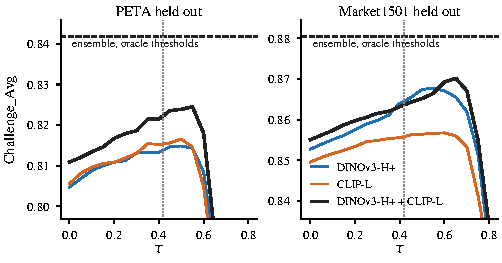
\includegraphics[width=\linewidth]{tau_rule.pdf}
\caption{Avg theo hệ số $\tau$ trên hai bộ dữ liệu giữ lại. Đường chấm đánh dấu giá trị của chúng tôi, đường gạch là cặp encoder với ngưỡng oracle.}
\label{fig:tau}
\end{figure}

\subsection{Kết hợp các encoder}
\label{sec:exp_design}

\Cref{tab:design} thử ba phương án thay cho cặp trọng số bằng nhau. Phương án thứ nhất thay đổi trọng số. Trên PETA, trọng số tốt nhất chính là trọng số bằng nhau. Trên Market1501, nó lệch về phía DINOv3, vốn đứng một mình đã tốt ngang mọi tỉ lệ trộn ở đó. Trọng số bằng nhau chỉ kém trọng số tốt nhất tối đa 0.11\pts{} trên cả hai bộ, trong khi dùng riêng một encoder có thể mất đến 0.91\pts. Vì vậy trọng số bằng nhau là lựa chọn an toàn khi chưa biết domain đích.

Phương án thứ hai thêm encoder thứ ba. Không ứng viên nào trong bốn ứng viên giúp được, kể cả MetaCLIP2 ViT-H/14, encoder lớn nhất chúng tôi thử. Encoder thứ ba phần lớn lặp lại một encoder đã có, và các false positive mà nó thêm vào gây thiệt hại ngang với phần nó sửa được.

Phương án thứ ba thay cặp bằng một encoder đơn cùng kích thước. Chúng tôi distill (tạm dịch: chưng cất) ensemble gồm DINOv3 ViT-H+, CLIP ViT-L/14 và MetaCLIP2 ViT-H/14 vào một student DINOv3 ViT-H+~\cite{hinton}. Riêng student đã chính xác ngang encoder đơn tốt nhất. Tuy nhiên khi ghép với CLIP, nó tăng ít hơn DINOv3 gốc, vì nó đã chép dự đoán của CLIP và không còn bất đồng với CLIP. \Cref{fig:cases} cho thấy vì sao sự bất đồng quan trọng. Với ba lô, DINOv3 tự tin và đúng, CLIP kém tự tin hơn và sai, nên trung bình đi theo DINOv3. Cùng hình đó cho thấy phép hiệu chỉnh hoạt động trên một thuộc tính hiếm là áo hồng.

\begin{table}[t]
\centering\small
\setlength{\tabcolsep}{4pt}
\begin{tabular}{@{}lcc@{}}
\toprule
Phương án & PETA & Market1501 \\
\midrule
Cặp, trọng số bằng nhau (của chúng tôi) & 82.33 & 86.35 \\
\quad trọng số DINOv3 0.4 & 82.30 & 86.23 \\
\quad trọng số DINOv3 0.6 & 82.29 & 86.46 \\
\midrule
+ MetaCLIP ViT-L/14 & 82.32 & -- \\
+ MetaCLIP2 ViT-H/14 & 82.27 & -- \\
+ AIMv2 ViT-L/14 & 82.16 & -- \\
+ SigLIP2 So400m/14 & 82.15 & -- \\
\midrule
student DINOv3 distill, đứng một mình & 82.00 & -- \\
student distill + CLIP & 82.21 & -- \\
\bottomrule
\end{tabular}
\caption{Đặt trọng số cho cặp, thêm encoder thứ ba, và distill ensemble vào một encoder.}
\label{tab:design}
\end{table}

\begin{figure*}[t]
\centering
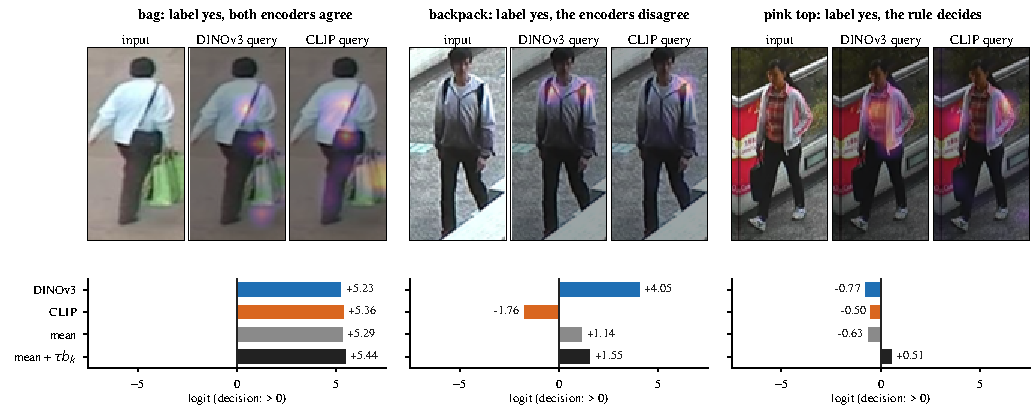
\includegraphics[width=\linewidth]{method_cases.pdf}
\caption{Ba trường hợp trên PETA với các encoder chưa từng thấy PETA. Trên là ảnh đầu vào và attention của query mỗi encoder cho thuộc tính được nêu. Dưới là logit của hai encoder, trung bình của chúng, và trung bình sau hiệu chỉnh prior.}
\label{fig:cases}
\end{figure*}

\subsection{Nên fine-tune sâu đến đâu}
\label{sec:exp_depth}

Chúng tôi cũng thử fine-tune sâu hơn, với bốn block đóng băng và hệ số decay 0.9 thay vì tám block và 0.75 (\cref{tab:depth}). Thiết lập này cho các block giữa của ViT-H+ learning rate lớn hơn khoảng hai mươi lần. Fine-tune sâu hơn làm tăng điểm source của mọi encoder. Trên dữ liệu giữ lại thì kết quả lẫn lộn. Nó giúp DINOv3, làm hại CLIP trên PETA, và chỉ thay đổi cặp trong phạm vi nhiễu. Trên tập test ẩn, cặp fine-tune sâu hơn đạt thấp hơn bản đã nộp 0.10\pts{} (\cref{sec:exp_test}). Như vậy khớp chặt hơn với các camera huấn luyện không mang lại lợi ích trên camera mới, và chúng tôi giữ thiết lập thận trọng.

\begin{table}[t]
\centering\small
\setlength{\tabcolsep}{3.2pt}
\resizebox{\columnwidth}{!}{%
\begin{tabular}{@{}lccc@{}}
\toprule
Mô hình & source & PETA giữ lại & Market1501 giữ lại \\
\midrule
DINOv3 ViT-H+ & 88.66 $\rightarrow$ 89.17 & 81.42 $\rightarrow$ 82.01 & 86.46 $\rightarrow$ 86.64 \\
CLIP ViT-L & 88.38 $\rightarrow$ 88.82 & 81.54 $\rightarrow$ 81.10 & 85.60 $\rightarrow$ 85.63 \\
Cặp (DINOv3 sâu hơn) & 89.14 $\rightarrow$ 89.35 & 82.33 $\rightarrow$ 82.51 & 86.35 $\rightarrow$ 86.42 \\
\bottomrule
\end{tabular}}
\caption{Fine-tune thận trọng $\rightarrow$ fine-tune sâu hơn.}
\label{tab:depth}
\end{table}

\subsection{Kết quả trên tập test ẩn}
\label{sec:exp_test}

\Cref{tab:test} liệt kê các bài nộp chính cùng điểm trên PETA giữ lại của cùng công thức. Điểm giữ lại xếp ba bài nộp đầu theo đúng thứ tự của tập test. Một DINOv3 ViT-L distill đơn đạt 79.12. Ensemble bốn mô hình thêm 0.63\pts. Cặp DINOv3 ViT-H+ và CLIP ViT-L, nhỏ hơn, thêm 0.22\pts{} nữa và là bài nộp tốt nhất của chúng tôi. Điểm giữ lại của v20 dùng student mười epoch thay cho student huấn luyện lâu hơn của nó. Fine-tune sâu hơn ở \cref{sec:exp_depth} tăng 0.18\pts{} trên PETA giữ lại, trong phạm vi nhiễu, và giảm 0.10\pts{} trên tập test. Trên tập test, hệ thống cuối cùng đạt mA 80.61 và instance F1 79.33, với precision 75.61 và recall 84.90.

\begin{table}[t]
\centering\small
\setlength{\tabcolsep}{3pt}
\resizebox{\columnwidth}{!}{%
\begin{tabular}{@{}llcc@{}}
\toprule
& Mô hình & PETA giữ lại & Test ẩn \\
\midrule
v13 & DINOv3 ViT-L/16 distill & 81.18 & 79.12 \\
v20 & student + DINOv3 ViT-L + CLIP-L + MetaCLIP2-H & 82.03 & 79.75 \\
v21 & DINOv3 ViT-H+ + CLIP ViT-L (của chúng tôi) & 82.33 & 79.97 \\
v22 & v21 với fine-tune sâu hơn & 82.51 & 79.87 \\
\bottomrule
\end{tabular}}
\caption{Các bài nộp chính vào UPAR 2027 Track~1.}
\label{tab:test}
\end{table}

%=====================================================================
\section{Kết luận}
\label{sec:conclusion}

Chúng tôi trình bày một hệ thống nhận dạng thuộc tính người đi bộ trên camera chưa thấy, gồm hai thành phần. Hai foundation encoder có cách pretrain khác nhau, chỉ fine-tune các block phía trên và được lấy trung bình, giúp cải thiện xếp hạng. Một phép hiệu chỉnh prior với một hệ số, suy ra từ metric, giúp cải thiện quyết định tại ngưỡng cố định. Mỗi thành phần thêm khoảng một điểm trên một bộ dữ liệu giữ lại, và phần tăng cộng dồn được. Các thí nghiệm cũng đưa ra hướng dẫn thực tế. Encoder đi cặp nên được chọn theo độ chính xác trên dữ liệu giữ lại, trọng số bằng nhau là đủ, còn ngưỡng hay mức fine-tune chỉnh trên dữ liệu huấn luyện không chuyển sang được camera mới. Lỗi lớn nhất còn lại đến từ quy ước gán nhãn của domain đích, thứ không thể học được nếu không có ít nhất một phần nhãn của nó.

\paragraph{Hạn chế.}\label{sec:limits} Phần lớn so sánh dùng một bộ dữ liệu giữ lại và một lần chạy cho mỗi thiết lập, và ước lượng nhiễu đến từ một encoder. \Cref{fig:arch,fig:cases} dùng các encoder ViT-L thuộc cùng hai họ, huấn luyện cùng thiết lập, vì phiên bản giữ lại của ViT-H+ đã nộp không được lưu. Phép hiệu chỉnh prior giả định tần suất huấn luyện được ước lượng từ dữ liệu đại diện.

\paragraph{Tác động rộng hơn.} Nhận dạng thuộc tính trên video giám sát, bao gồm tuổi và giới tính, có thể hỗ trợ việc theo dõi cá nhân. Chúng tôi chỉ báo cáo kết quả kỹ thuật và không công bố mô hình huấn luyện trên dữ liệu giám sát.

{\small
\bibliographystyle{ieeenat_fullname}
\bibliography{refs}
}

%=====================================================================
\clearpage
\appendix
\section{Cấu hình huấn luyện}
\label{app:config}

Hai encoder dùng cùng thiết lập. Bộ tối ưu là AdamW với learning rate $5\cdot10^{-5}$ ở block cuối, layer decay 0.75, learning rate của head lớn gấp mười lần, weight decay 0.05 và batch size 64. Lịch learning rate dạng cosine với nửa epoch warm-up và kéo dài ba epoch. Huấn luyện dùng stochastic depth 0.1, độ chính xác hỗn hợp bf16 và trung bình trượt mũ (EMA) của trọng số với hệ số 0.9995, đây là mô hình dùng khi test. Query head có một tầng, tám attention head, tỉ lệ MLP bằng hai và dropout 0.1. Augmentation gồm giảm độ phân giải ngẫu nhiên để mô phỏng ảnh mờ, lật ngang, đệm biên mười pixel rồi cắt ngẫu nhiên, thay đổi độ sáng, độ tương phản và độ bão hoà mà không đổi sắc độ, làm mờ Gauss và xoá vùng ngẫu nhiên. Tần suất thuộc tính $\pi_k$ được giới hạn trong $[10^{-3},1-10^{-3}]$, và nhãn mà một bộ dữ liệu không gán được che khỏi loss. Khi test, cả hai encoder đọc cùng ảnh cắt đổi kích thước về $224\times112$, và cặp encoder xử lý 29{,}248 ảnh test trong khoảng bốn phút trên một GPU NVIDIA A10.

\end{document}

